% =============================================================================
% EventSPD — Architecture Document
% =============================================================================
\documentclass[11pt, letterpaper]{article}

\usepackage[utf8]{inputenc}
\usepackage[T1]{fontenc}
\usepackage{amsmath, amssymb, amsfonts}
\usepackage{mathtools}
\usepackage{booktabs}
\usepackage{graphicx}
\usepackage{xcolor}
\usepackage[margin=1in]{geometry}
\usepackage{hyperref}
\usepackage{cleveref}
\usepackage{enumitem}
\usepackage{caption}
\usepackage{multirow}
\usepackage[numbers,sort&compress]{natbib}
\usepackage{microtype}
\usepackage{tikz}
\usetikzlibrary{arrows.meta, positioning, calc, fit, backgrounds}

\hypersetup{colorlinks=true, linkcolor=blue!70!black,
    citecolor=green!50!black, urlcolor=blue!70!black}

\newcommand{\Ft}{F_t}
\newcommand{\Gt}{G_t}
\newcommand{\R}{\mathbb{R}}
\newcommand{\softplus}{\operatorname{softplus}}
\newcommand{\GELU}{\operatorname{GELU}}
\newcommand{\LN}{\operatorname{LN}}
\newcommand{\FFN}{\operatorname{FFN}}
\newcommand{\TopR}{\operatorname{Top\text{-}R}}

% =============================================================================
\title{\textbf{EventSPD: Sparse Query-Point Depth from Event Cameras}\\[6pt]
\large Architecture Document (based on research plan v12)}
\author{Yincheng Zhou \\ Formatted by Claude Code}
\date{February 2026}

\begin{document}
\maketitle

% =============================================================================
\section{Motivation}

Every existing event-camera depth method~\cite{hidalgo2020e2depth,
bartolomei2025depthanyevent} produces a dense $H{\times}W$ depth map. Yet many
downstream tasks---SLAM keypoint tracking, grasping, obstacle avoidance---need
depth at only a sparse set of pixels ($K \ll HW$). Dense decoding wastes both
latency and power on the majority of pixels that are never used.

We propose \textbf{EventSPD}, which predicts depth only at user-specified query
pixels. Inference decomposes as:
\begin{equation}
    T(K) = \underbrace{T_{\text{precompute}}}_{\text{shared, } \sim\!6\text{ ms}}
    + \underbrace{\beta \cdot K}_{\sim\!5\,\mu\text{s / query}}
\end{equation}
At $K{=}256$ on an RTX~4090, this gives ${\sim}7.8$\,ms total
(estimated from MACs calculation, $2.9{\times}$ faster than the dense baseline combining
F$^3$~\cite{das2025f3}---a predictive event-camera feature encoder---and
DAv2~\cite{yang2024dav2}---a dense monocular depth decoder---at
${\sim}23$\,ms).

No published work targets sparse query-point depth from events. The closest RGB
work is InfiniDepth~\cite{infinidepth2026} (LIIF-style~\cite{chen2021liif}
queries), which lacks attention routing and deformable sampling.


% =============================================================================
\section{Background and Related Work}

\paragraph{RGB depth foundations.}
MiDaS~\cite{ranftl2020midas} introduced mixed-dataset zero-shot transfer.
DPT~\cite{ranftl2021dpt} added ViT backbones with token reassembly.
Depth Anything V2~\cite{yang2024dav2} (NeurIPS 2024) scales this further with
synthetic pre-training. ZoeDepth~\cite{bhat2023zoedepth},
Metric3D v2~\cite{hu2024metric3d}, Marigold~\cite{ke2024marigold}, and
UniDepth~\cite{piccinelli2024unidepth} represent further advances. All decode
densely.

\paragraph{Event-camera depth.}
E2Depth~\cite{hidalgo2020e2depth} uses recurrent ConvLSTM~\cite{shi2015convlstm}
for dense event depth. Depth AnyEvent~\cite{bartolomei2025depthanyevent}
(ICCV 2025) distills DAv2 into an event encoder with a recurrent variant.
DERD-Net (NeurIPS 2025) uses a lightweight GRU. F$^3$~\cite{das2025f3}
provides a predictive event representation at 120\,Hz (HD). All produce dense
output.

\paragraph{Query-based decoders.}
DETR~\cite{carion2020detr} and Deformable DETR~\cite{zhu2021deformable}
decode object queries via cross-attention into encoder features.
SAM~\cite{kirillov2023sam} extends this to promptable segmentation.
Perceiver IO~\cite{jaegle2022perceiverio} generalizes to arbitrary outputs.
Our decoder follows the same principle: pre-computed features as static KV
context, with each query point cross-attending through multiple layers.


% =============================================================================
\section{Architecture}

\subsection*{Overview}

EventSPD decomposes inference into two phases:

\begin{center}
\small
\begin{tabular}{lp{9cm}}
\toprule
\textbf{Phase} & \textbf{Description} \\
\midrule
\textbf{A. Shared Precompute}
    & Runs \emph{once per event window}. Encodes raw events into a
      multi-scale feature pyramid (4 levels), applies temporal
      recurrence, and pre-computes KV projections shared across all
      queries. \\
\textbf{B. Per-Query Decoder}
    & Runs \emph{independently for each of $K$ queries} in parallel.
      Five stages progressively refine a query embedding: local
      feature gathering $\to$ local cross-attention $\to$ global
      cross-attention with routing $\to$ deformable multi-scale
      sampling $\to$ fused cross-attention $\to$ depth prediction. \\
\bottomrule
\end{tabular}
\end{center}

\begin{figure}[h]
\centering
\resizebox{\textwidth}{!}{%
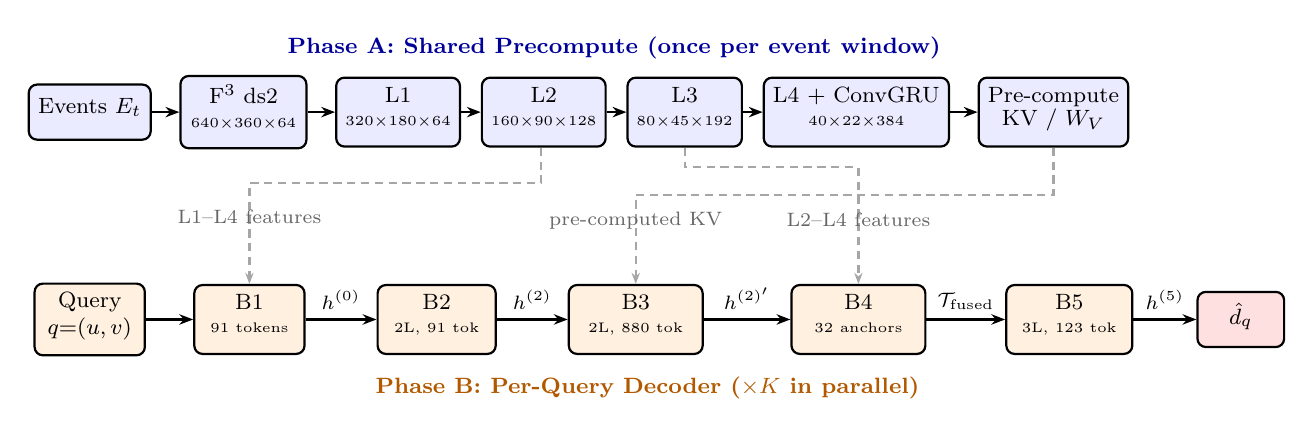
\begin{tikzpicture}[
    block/.style={draw, rounded corners=3pt, minimum height=0.7cm,
        text depth=0.15cm, font=\footnotesize, align=center, thick},
    phasea/.style={block, fill=blue!8},
    phaseb/.style={block, fill=orange!12},
    arr/.style={-{Stealth[length=5pt]}, thick},
    feed/.style={-{Stealth[length=4pt]}, thick, densely dashed, gray!70},
    lbl/.style={font=\tiny, gray!80},
]

% ---- Phase A row ----
\node[phasea, minimum width=1.4cm] (evt)
    {Events $E_t$};
\node[phasea, right=0.35 of evt, minimum width=1.6cm] (f3)
    {F$^3$ ds2\\[-1pt]{\tiny $640{\times}360{\times}64$}};
\node[phasea, right=0.35 of f3, minimum width=1.3cm] (l1)
    {L1\\[-1pt]{\tiny $320{\times}180{\times}64$}};
\node[phasea, right=0.25 of l1, minimum width=1.3cm] (l2)
    {L2\\[-1pt]{\tiny $160{\times}90{\times}128$}};
\node[phasea, right=0.25 of l2, minimum width=1.3cm] (l3)
    {L3\\[-1pt]{\tiny $80{\times}45{\times}192$}};
\node[phasea, right=0.25 of l3, minimum width=1.8cm] (l4)
    {L4 + ConvGRU\\[-1pt]{\tiny $40{\times}22{\times}384$}};
\node[phasea, right=0.35 of l4, minimum width=1.6cm] (kv)
    {Pre-compute\\[-1pt]KV / $W_V$};

% Phase A arrows
\draw[arr] (evt) -- (f3);
\draw[arr] (f3) -- (l1);
\draw[arr] (l1) -- (l2);
\draw[arr] (l2) -- (l3);
\draw[arr] (l3) -- (l4);
\draw[arr] (l4) -- (kv);

% Phase A label
\node[font=\footnotesize\bfseries, anchor=south, blue!60!black]
    at ($(l2)!0.5!(l3) + (0, 0.55)$)
    {Phase A: Shared Precompute (once per event window)};

% ---- Phase B row ----
\node[phaseb, below=1.8cm of evt, minimum width=1.4cm] (q)
    {Query\\$q{=}(u,v)$};
\node[phaseb, right=0.6 of q, minimum width=1.4cm] (b1)
    {B1\\[-1pt]{\tiny 91 tokens}};
\node[phaseb, right=0.9 of b1, minimum width=1.5cm] (b2)
    {B2\\[-1pt]{\tiny 2L, 91 tok}};
\node[phaseb, right=0.9 of b2, minimum width=1.7cm] (b3)
    {B3\\[-1pt]{\tiny 2L, 880 tok}};
\node[phaseb, right=1.1 of b3, minimum width=1.7cm] (b4)
    {B4\\[-1pt]{\tiny 32 anchors}};
\node[phaseb, right=1.0 of b4, minimum width=1.6cm] (b5)
    {B5\\[-1pt]{\tiny 3L, 123 tok}};
\node[block, right=0.8 of b5, fill=red!12, minimum width=1.1cm] (d)
    {$\hat{d}_q$};

% Phase B arrows (labels use \scriptsize for readability)
\draw[arr] (q) -- (b1);
\draw[arr] (b1) -- (b2)
    node[midway, above, font=\scriptsize] {$h^{(0)}$};
\draw[arr] (b2) -- (b3)
    node[midway, above, font=\scriptsize] {$h^{(2)}$};
\draw[arr] (b3) -- (b4)
    node[midway, above, font=\scriptsize] {$h^{(2)'}$};
\draw[arr] (b4) -- (b5)
    node[midway, above, font=\scriptsize] {$\mathcal{T}_{\text{fused}}$};
\draw[arr] (b5) -- (d)
    node[midway, above, font=\scriptsize] {$h^{(5)}$};

% Phase B label
\node[font=\footnotesize\bfseries, anchor=north, orange!70!black]
    at ($(b2)!0.5!(b4) + (0, -0.6)$)
    {Phase B: Per-Query Decoder ($\times K$ in parallel)};

% ---- Cross-phase feeds (single clean arrows per connection) ----

% L1--L4 features → B1: anchor from midpoint of L1–L3, drop to B1
\coordinate (a2mid) at ($(l1.south)!0.5!(l3.south)$);
\draw[feed] (a2mid) -- ++(0,-0.45)
    -| (b1.north)
    node[pos=0.75, above, font=\scriptsize, black!60]
    {L1--L4 features};

% Pre-computed KV → B3: drop from KV, route left to B3
\draw[feed] (kv.south) -- ++(0,-0.6)
    -| (b3.north)
    node[pos=0.75, above, font=\scriptsize, black!60]
    {pre-computed KV};

% L2--L4 pre-projected features → B4: anchor from L3, drop to B4
\draw[feed] (l3.south) -- ++(0,-0.25)
    -| (b4.north)
    node[pos=0.8, above, font=\scriptsize, black!60]
    {L2--L4 features};

\end{tikzpicture}
}%
\caption{EventSPD architecture overview. Phase~A (top) runs once per
event window, producing a 4-level feature pyramid and pre-computed KV
projections. Phase~B (bottom) runs independently for each of $K$ query
pixels: five stages progressively refine a query embedding into a depth
prediction. Dashed arrows show feature feeds from Phase~A into Phase~B
stages.}
\label{fig:arch}
\end{figure}

\paragraph{Design principles and references.}
The architecture draws on several established ideas, combined in a
novel way for sparse event-camera depth:

\begin{center}
\small
\begin{tabular}{lp{5.2cm}l}
\toprule
\textbf{Component} & \textbf{What we use} & \textbf{Reference} \\
\midrule
Event encoding
    & F$^3$ ds2 (predictive features, 120\,Hz)
    & \cite{das2025f3} \\
Local backbone (L1--L2)
    & Large-kernel depthwise conv + GRN
    & \cite{woo2023convnextv2,ding2024unireplknet} \\
Mid-range backbone (L3)
    & Shifted window self-attention
    & \cite{liu2021swin} \\
Temporal state (L4)
    & Depthwise-separable ConvGRU
    & \cite{bartolomei2025depthanyevent} \\
Per-layer KV projections
    & Fresh KV per decoder layer
    & \cite{carion2020detr,kirillov2023sam} \\
Deformable sampling (B4)
    & Multi-scale offsets + grid-sample
    & \cite{zhu2021deformable} \\
Static KV context (B5)
    & Uncompressed features as KV across layers
    & \cite{jaegle2022perceiverio} \\
Feature distillation
    & Cosine similarity to frozen DAv2
    & \cite{bartolomei2025depthanyevent} \\
Query-point paradigm
    & Decode only at requested pixels
    & \cite{chen2021liif,kirillov2020pointrend} \\
\bottomrule
\end{tabular}
\end{center}

\paragraph{End-to-end data flow.}
The full pipeline proceeds as follows:

\begin{center}
\small
\begin{tabular}{rp{6.5cm}l}
\toprule
\textbf{Step} & \textbf{Operation} & \textbf{Output} \\
\midrule
A1 & F$^3$ ds2: raw events $\to$ feature tensor
    & $\Ft \in \R^{640 \times 360 \times 64}$ \\
A2 & Wide pyramid backbone
      (ConvNeXt $\to$ Swin $\to$ SelfAttn $\to$ ConvGRU)
    & L1--L4 feature maps \\
A3 & Pre-compute KV projections for B3; $W_V$ for B4
    & Shared KV tables \\
A4 & Global calibration from mean-pooled L4
    & Scale $s_t$, shift $b_t$ \\
\midrule
B1 & Gather multi-scale tokens around query $q$
    & $\mathcal{T}_{\text{uni}} \!\in\! \R^{91 \times d}$, $h^{(0)}$ \\
B2 & Local cross-attn (2L) over 91 tokens
    & $h^{(2)}$ (local-aware) \\
B3 & Global cross-attn (2L) over 880 L4 tokens + routing
    & $h^{(2)'}$ + 32 anchors \\
B4 & Deformable multi-scale read at 32 anchors
    & $\mathcal{T}_{\text{fused}} \!\in\! \R^{123 \times d}$ \\
B5 & Fused cross-attn (3L) over 123 tokens + depth MLP
    & $\hat{d}_q$ \\
\bottomrule
\end{tabular}
\end{center}

\paragraph{Key numbers.}
\begin{center}
\small
\begin{tabular}{ll}
\toprule
\textbf{Quantity} & \textbf{Value} \\
\midrule
Core dimension $d$ & 192 \\
Feature pyramid & 4 levels: 64 / 128 / 192 / 384 channels at
    strides 4 / 8 / 16 / 32 \\
Cross-attention layers & 7 total (2 in B2 + 2 in B3 + 3 in B5);
    6 heads, $d_h{=}32$ \\
Lookups per query & 2,396 (92 local + 2,304 deformable) \\
MACs per query & $\sim$51.1M ($\sim$4.9\,$\mu$s wall-clock) \\
Total parameters & $\sim$11.1M (7.7M backbone + 3.4M decoder) \\
Precompute latency & $\sim$6.15\,ms (F$^3$ 4.5\,ms + backbone 1.55\,ms + 0.10\,ms) \\
\bottomrule
\end{tabular}
\end{center}

% --- Phase A -----------------------------------------------------------------
\subsection*{Phase A: Shared Precompute}

\subsubsection*{A1. Event Encoding (F$^3$ ds2)}

F$^3$~\cite{das2025f3} encodes a fixed-duration \emph{event window}
$E_t$ (all events accumulated within one time step at 120\,Hz) into a
dense feature tensor. We use the \textbf{ds2} (``down-sample $2{\times}$'')
configuration, which applies stride-2 in the first stage with 64 channels
(vs.\ ds1's 32 channels at full $1280{\times}720$):
\begin{equation}
    \Ft = \mathcal{F}^{\text{ds2}}(E_t)
    \;\in\; \R^{640 \times 360 \times 64}
    \qquad (\sim\!4.5\text{ ms})
\end{equation}
ds2 halves spatial resolution and memory traffic relative to ds1. The
resulting 59\,MB feature map fits the RTX 4090 L2 cache (72\,MB). ds2 requires training first.

\subsubsection*{A2. Wide Pyramid Backbone}

Four-level features at strides $[4, 8, 16, 32]$ and channels
$[64, 128, 192, 384]$:

\begin{center}
\small
\begin{tabular}{llll}
\toprule
\textbf{Level} & \textbf{Blocks} & \textbf{Output} & \textbf{Params} \\
\midrule
Stem   & Conv $k{=}3$, $s{=}2$ + LN & $320{\times}180{\times}64$ & 37K \\
L1     & 2$\times$ ConvNeXt V2, $k{=}7$~\cite{woo2023convnextv2} & $320{\times}180{\times}64$ & 74K \\
L2     & 3$\times$ ConvNeXt V2, $k{=}13$~\cite{ding2024unireplknet} & $160{\times}90{\times}128$ & 435K \\
L3     & 4$\times$ Swin~\cite{liu2021swin}, $w{=}8$ & $80{\times}45{\times}192$ & 1,778K \\
L4     & 2$\times$ Full self-attn & $40{\times}22{\times}384$ & 3,542K \\
ConvGRU & 3 gates, DW-sep $k{=}3$ & $40{\times}22{\times}384$ & 886K \\
\midrule
\multicolumn{3}{l}{\textbf{Total backbone}} & \textbf{7,179K} \\
\bottomrule
\end{tabular}
\end{center}

\textbf{Design rationale.} L1--L2 use ConvNeXt with large kernels for local
depth features at high resolution. L3 uses windowed attention for mid-range
context. L4 uses full self-attention (880 tokens, trivially cheap) for global
scene understanding. The ConvGRU at L4 integrates temporal state across event
windows~\cite{bartolomei2025depthanyevent,shi2015convlstm} (standard
ConvGRU formulation; we show only the state update for brevity):
\begin{equation}
    \Gt^{(4)} = (1{-}z_t) \odot h_{t-1} + z_t \odot \tilde{h}_t
\end{equation}
where $z_t$ is the update gate, $\tilde{h}_t$ the candidate (both
computed via depthwise-separable $3{\times}3$ convolutions), and
$h_0{=}0$.
Placing recurrence only at L4 minimizes cost (${\sim}0.8$G MACs) while
maximizing impact (global receptive field).

Total backbone cost: ${\sim}25.8$G MACs, ${\sim}1.55$ ms.

\subsubsection*{A3. Pre-Computed Projections}

Pre-computed once per frame and shared across all queries:

\begin{center}
\small
\begin{tabular}{llll}
\toprule
\textbf{Target} & \textbf{Projection} & \textbf{Shape} & \textbf{Params} \\
\midrule
B3 KV ($\ell{=}1,2$)~\cite{carion2020detr,kirillov2023sam}
    & $W_K^{(\ell)}, W_V^{(\ell)}$ per layer
    & $384{\to}192$ & 296K \\
B4 anchor ($W_g$)
    & L4 feature $\to$ conditioning
    & $384{\to}192$ & 74K \\
B4 value ($W_V$)
    & Per-level pre-proj~\cite{zhu2021deformable}
    & L2: $128{\to}192$, L3: id, L4: $384{\to}192$ & 136K \\
\midrule
\multicolumn{3}{l}{\textbf{Total A3}} & \textbf{506K} \\
\bottomrule
\end{tabular}
\end{center}

\subsubsection*{A4. Calibration}

Global scale and shift for converting the decoder's raw output into
metric depth, derived from mean-pooled L4:
\begin{align}
    \bar{G}_t^{(4)} &= \frac{1}{HW}\sum_{i} \Gt^{(4)}[i]
    \;\in\; \R^{384} \\
    s_t &= \softplus\!\bigl(W_s \, \bar{G}_t^{(4)} + b_s\bigr),
    \qquad
    b_t = W_b \, \bar{G}_t^{(4)} + b_b
\end{align}
where $W_s, W_b \in \R^{1 \times 384}$ are linear heads (${\sim}0.8$K
params each). These are used in B5's depth prediction
(Eq.~\ref{eq:depth}).




% --- Phase B -----------------------------------------------------------------
\subsection*{Phase B: Per-Query Decoder ($d = 192$)}

\paragraph{Notation conventions.}
Layer indices $\ell$ are local to each stage (B2 and B3 each have
$\ell{=}1,2$; B5 has $\ell{=}1,2,3$). In B3, $h^{(2)}$ denotes
in-place updates starting from B2's output; the final result is written
$h^{(2)'}$ to distinguish it. All Fourier positional encodings are
written $\phi_n(\cdot)$ where $n$ is the number of frequencies (output
dimensionality $= 4n$). RPE denotes learned relative position
embeddings.

\subsubsection*{B1. Token Construction}

Gathers multi-scale features around query $q = (u,v)$:

\begin{center}
\small
\begin{tabular}{lrp{3.8cm}p{4.5cm}l}
\toprule
\textbf{Scale} & \textbf{Tok.} & \textbf{Grid / Source}
    & \textbf{Projection} & \textbf{Embed.} \\
\midrule
L1 (stride 4)  & 32 & 24 grid (5$\times$5 excl.\ center) + 8 adaptive
    & MLP: $h_\delta{=}\GELU(W_{\text{loc}}[f_\delta;\phi_4(\delta)])$
    & $e_{L1}$ \\
L2 (stride 8)  & 25 & 5$\times$5 grid
    & $W_{v2}$: $128{\to}192$ & $e_{L2}$ + RPE \\
L3 (stride 16) & 25 & 5$\times$5 grid
    & identity ($192{=}d$) & $e_{L3}$ + RPE \\
L4 (stride 32) & 9  & 3$\times$3 grid
    & $W_{v4}$: $384{\to}192$ & $e_{L4}$ + RPE \\
\midrule
\textbf{Total}  & \textbf{91} & & & \\
\bottomrule
\end{tabular}
\end{center}

The combined token set:
\begin{equation}
    \mathcal{T}_{\text{uni}} = [\,
    \underbrace{t^{(1)}_{1:32}}_{L1}\,;\;
    \underbrace{t^{(2)}_{1:25}}_{L2}\,;\;
    \underbrace{t^{(3)}_{1:25}}_{L3}\,;\;
    \underbrace{t^{(4)}_{1:9}}_{L4}\,]
    \;\in\; \R^{91 \times 192}
\end{equation}

\textbf{Query seed:} $h^{(0)} = W_q[f_q^{(1)};\,\phi_8(q)] \in \R^{192}$,
where $f_q^{(1)} \in \R^{64}$ is the bilinear-sampled L1 center feature
and $\phi_8(q) \in \R^{32}$ is a Fourier encoding of the normalized query
pixel coordinate $(u/W, v/H)$ with 8 frequencies.

\textit{B1 cost:} 142K params, 92 bilinear lookups, $\sim$2M MACs.

\subsubsection*{B2. Local Multi-Scale Cross-Attention}

Two-layer cross-attention decoder ($\ell = 1, 2$) with $h^{(0)}$ as
initial query and $\mathcal{T}_{\text{uni}}$ (91 tokens) as context.
6 heads, $d_h{=}32$, FFN $192{\to}768{\to}192$.

\textbf{Per-layer KV projections} (DETR/SAM/Perceiver IO
convention~\cite{carion2020detr,kirillov2023sam,jaegle2022perceiverio}):
\begin{align}
    K^{(\ell)} &= W_K^{(\ell)} \, \LN_{\text{kv}}(\mathcal{T}_{\text{uni}}),
    \quad
    V^{(\ell)} = W_V^{(\ell)} \, \LN_{\text{kv}}(\mathcal{T}_{\text{uni}})
    \;\in\; \R^{91 \times d}
\end{align}
where $\LN_{\text{kv}}$ is shared across B2 layers (normalizes
heterogeneous token scales once); $W_K^{(\ell)}, W_V^{(\ell)} \in
\R^{d \times d}$ are per-layer.

\textbf{Pre-LN decoder} (each layer = cross-attention + FFN with
residuals):
\begin{align}
    h^{(\ell)} &\leftarrow h^{(\ell-1)} +
        \operatorname{MHCrossAttn}^{(\ell)}\!\bigl(
        Q{=}\LN_q^{(\ell)}(h^{(\ell-1)}),\;
        K{=}K^{(\ell)},\;
        V{=}V^{(\ell)}\bigr) \\
    h^{(\ell)} &\leftarrow h^{(\ell)} +
        \FFN^{(\ell)}\!\bigl(\LN_{\text{ff}}^{(\ell)}(h^{(\ell)})\bigr)
\end{align}

Output: $h^{(2)} \in \R^d$---local-aware query representation encoding
fine L1 texture, mid-level L2/L3 structure, and coarse L4 context from
the query neighborhood. B2 is the costliest stage because the 91 tokens
are per-query (KV projection runs per query), unlike B3's pre-computed
KV.

\textit{B2 cost:} 891K params (2$\times$ $W_Q/W_K/W_V/W_O$ $\sim$296K
+ 2$\times$ FFN $\sim$592K + LNs $\sim$3K), $\sim$14.2M MACs.

\subsubsection*{B3. Global L4 Cross-Attention + Routing}

Two-layer cross-attention ($\ell = 1, 2$) into the full L4 feature map
(880 tokens). KV pairs are \emph{pre-computed in Phase A}
($K_t^{(\ell)}, V_t^{(\ell)} \in \R^{880 \times d}$ from A3, per-layer
projections $W_K^{(\ell)}, W_V^{(\ell)} \in \R^{d \times 384}$).
Per-query cost is only Q projection + attention + FFN---no KV
recomputation.

\textbf{Pre-LN decoder} (same structure as B2; $h^{(2)}$ from B2 is
updated in-place across B3's two layers):
\begin{align}
    h^{(2)} &\leftarrow h^{(2)} +
        \operatorname{MHCrossAttn}^{(\ell)}\!\bigl(
        Q{=}\LN_q^{(\ell)}(h^{(2)}),\;
        K{=}K_t^{(\ell)},\;
        V{=}V_t^{(\ell)}\bigr) \\
    h^{(2)} &\leftarrow h^{(2)} +
        \FFN^{(\ell)}\!\bigl(\LN^{(\ell)}(h^{(2)})\bigr)
\end{align}
6 heads, $d_h{=}32$, FFN $192{\to}768{\to}192$.
After 2 layers the result is denoted $h^{(2)'} \in \R^d$---enriched
with global scene context.

\textbf{Attention-based routing} (parameter-free). Average B3's
\emph{second-layer} attention weights across heads, select top-$R$:
\begin{equation}
    \bar{\alpha}_q = \frac{1}{H}\sum_{h=1}^{H} \alpha_{q,h}
    \;\in\; \R^{880},
    \qquad
    R_q = \TopR(\bar{\alpha}_q,\; R{=}32)
    \qquad \text{(3.6\% selection)}
\end{equation}
Each $r \in R_q$ maps to pixel coordinate $\mathbf{p}_r$ via L4 grid
geometry ($40{\times}22$, stride 32). Gradient flow through the
discrete selection uses a straight-through estimator.

Output: $h^{(2)'}$ (globally enriched) + 32 anchor positions for B4.

\textit{B3 cost:} 740K params, $\sim$1.4M MACs per query. Cheap because
KV is pre-computed and shared across all queries.

\subsubsection*{B4. Deformable Multi-Scale Read + Token Fusion}

For each anchor $r \in R_q$ (32 from B3), predict sampling offsets and
importance weights, then read from the multi-scale pyramid via bilinear
grid-sample~\cite{zhu2021deformable}:

\begin{center}
\small
\begin{tabular}{ll}
\toprule
\textbf{Hyperparameter} & \textbf{Value} \\
\midrule
Heads ($H$)          & 6 \\
Levels ($L$)         & 3 (L2, L3, L4) \\
Samples / head / level ($M$) & 4 \\
Anchors ($R$)        & 32 (from B3 routing) \\
Total lookups        & $32 \times 6 \times 3 \times 4 = 2{,}304$ \\
\bottomrule
\end{tabular}
\end{center}

\textbf{Conditioning.} Each anchor is conditioned on the query state,
anchor content, and spatial offset:
\begin{align}
    \Delta\mathbf{p}_r &= \mathbf{p}_r - q
    \qquad\text{(query-to-anchor offset in pixels)} \\
    u_r &= \LN\!\bigl(\GELU(
        W_u\,[h^{(2)'};\; g_r;\; \phi_8(\Delta\mathbf{p}_r)] + b_u
    )\bigr)
    \;\in\; \R^d
\end{align}
where $g_r = W_g \, \Gt^{(4)}[\mathbf{p}_r^{(4)}] \in \R^d$ is the
anchor's L4 feature (pre-projected $384{\to}192$ in A3), and
$\phi_8(\Delta\mathbf{p}_r) \in \R^{32}$ is a Fourier encoding
(8 frequencies) of the normalized offset
$[\Delta u/W,\; \Delta v/H]$.
Input dimension: $d + d + 32 = 416$.

\textbf{Offset and weight prediction.} Two shared linear heads from the
conditioning:
\begin{align}
    \Delta p_{r,h,\ell,m} &= W^\Delta \, u_r + b^\Delta
    \;\in\; \R^{H \times L \times M \times 2}
    \quad\text{(offsets, $d{\to}144$)} \\
    \beta_{r,h,\ell,m} &= W^a \, u_r + b^a
    \;\in\; \R^{H \times L \times M}
    \quad\text{(weights, $d{\to}72$)}
\end{align}
Offsets are unbounded (no tanh), following Deformable
DETR~\cite{zhu2021deformable}. Zero-initialized with $0.1{\times}$ LR.

\textbf{Sampling with per-level normalization.} Each offset is
normalized by the spatial extent $S_\ell$ of level $\ell$ (making
offsets scale-invariant):
\begin{align}
    p_{\text{sample}} &= \mathbf{p}_r^{(\ell)} +
        \frac{\Delta p_{r,h,\ell,m}}{S_\ell} \\
    f_{r,h,\ell,m} &=
        \operatorname{GridSample}\!\bigl(
        \hat{F}_t^{(\ell)},\;
        \operatorname{Normalize}(p_{\text{sample}})
        \bigr)
\end{align}
where $\mathbf{p}_r^{(\ell)} = \mathbf{p}_r / s_\ell$ maps the anchor
to level-$\ell$ native coordinates, $\hat{F}_t^{(\ell)}$ are the
pre-projected features (already at $d{=}192$ from A3's $W_V$), and
$S_\ell \in \{160, 80, 40\}$ for L2--L4.

\textbf{Multi-head per-anchor aggregation.} Per-head softmax over
$L{\times}M{=}12$ samples, weighted sum, then concat + output
projection:
\begin{align}
    a_{r,h,\ell,m} &= \frac{\exp(\beta_{r,h,\ell,m})}
        {\sum_{\ell',m'} \exp(\beta_{r,h,\ell',m'})},
    \qquad
    \tilde{h}_{r,h} = \sum_{\ell,m}
        a_{r,h,\ell,m} \, v_{r,h,\ell,m} \\
    h_r &= W_O\,[\tilde{h}_{r,1};\;\ldots;\;\tilde{h}_{r,H}] + b_O
    \;\in\; \R^d
\end{align}
where $v_{r,h,\ell,m} \in \R^{d/H}$ is the head-partitioned feature
from $f_{r,h,\ell,m}$.

\textbf{Token fusion.} The 32 deformable tokens are appended with a
type embedding $e_{\text{deform}} \in \R^d$:
\begin{equation}
    \mathcal{T}_{\text{fused}} = [\,\mathcal{T}_{\text{uni}};\;
    h_{r_1}{+}e_{\text{deform}};\;\ldots;\;
    h_{r_{32}}{+}e_{\text{deform}}\,]
    \;\in\; \R^{123 \times d}
\end{equation}
Budget: $32 \times 72 = \textbf{2{,}304}$ deformable lookups (all
remote).

\textit{B4 cost:} 159K params (conditioning $\sim$80K + offsets
$\sim$28K + weights $\sim$14K + $W_O$ $\sim$37K), $\sim$5.1M MACs.
Dominates \textbf{wall-clock} (51\%) due to scattered memory reads
despite only 10\% of compute.

\subsubsection*{B5. Fused Cross-Attention + Depth Head}

Three-layer cross-attention decoder ($\ell = 1, 2, 3$, local to B5)
with $h^{(2)'}$ as initial query and $\mathcal{T}_{\text{fused}}$
(123 tokens) as KV. Same architecture as B2 (6 heads, $d_h{=}32$, FFN
$192{\to}768{\to}192$). The 91 local tokens remain as
\emph{uncompressed} reference in KV---following DETR/SAM's convention
of static context across decoder
layers~\cite{carion2020detr,kirillov2023sam}.

\textbf{Per-layer KV projections} (independent from B2):
\begin{align}
    K^{(\ell)} &= W_K^{(\ell)} \, \LN_{\text{kv2}}(\mathcal{T}_{\text{fused}}),
    \quad
    V^{(\ell)} = W_V^{(\ell)} \, \LN_{\text{kv2}}(\mathcal{T}_{\text{fused}})
    \;\in\; \R^{123 \times d}
\end{align}

\textbf{Pre-LN decoder} (same structure as B2):
\begin{align}
    h^{(\ell)} &\leftarrow h^{(\ell-1)} +
        \operatorname{MHCrossAttn}^{(\ell)}\!\bigl(
        Q{=}\LN_q^{(\ell)}(h^{(\ell-1)}),\;
        K{=}K^{(\ell)},\;
        V{=}V^{(\ell)}\bigr) \\
    h^{(\ell)} &\leftarrow h^{(\ell)} +
        \FFN^{(\ell)}\!\bigl(\LN_{\text{ff}}^{(\ell)}(h^{(\ell)})\bigr)
\end{align}
Output after 3 layers: $h^{(5)} \coloneqq h_{\text{B5}}^{(3)}$ (we
write $h^{(5)}$ to reflect the total decoder depth: 2 B2 + 3 B5 = 5
cross-attention layers).

\textbf{Depth prediction:}
\begin{align}
    z_q &= W_{z2} \cdot \GELU(W_{z1}\,h^{(5)} + b_{z1}) + b_{z2}
    \qquad\text{(MLP $192{\to}384{\to}1$)} \label{eq:depth} \\
    \hat{d}_q &= \frac{1}{\underbrace{\softplus(s_t \, z_q + b_t) + \varepsilon}_{\hat{\rho}_q \;=\; \text{predicted inverse depth}}}
\end{align}
where $s_t, b_t$ are the global calibration parameters from A4.

\textit{B5 cost:} 1,411K params (3$\times$ $W_Q/W_K/W_V/W_O$
$\sim$444K + 3$\times$ FFN $\sim$888K + depth MLP $\sim$74K + LNs
$\sim$5K), $\sim$28.4M MACs.

\subsubsection*{Summary}

\begin{equation}
    h^{(0)} \xrightarrow[\text{2L, 91 tok}]{\text{B2}}
    h^{(2)} \xrightarrow[\text{2L, 880 tok}]{\text{B3}}
    h^{(2)'} \xrightarrow[\text{3L, 123 tok}]{\text{B5}}
    h^{(5)} \to \hat{d}_q
\end{equation}

\begin{center}
\small
\begin{tabular}{lrrr}
\toprule
\textbf{Stage} & \textbf{Params} & \textbf{Lookups} & \textbf{MACs/query} \\
\midrule
B1: Token construction & 142K & 92 & 2.0M \\
B2: Local cross-attn (2L, 91 tok) & 891K & --- & 14.2M \\
B3: Global cross-attn (2L, 880 tok) & 740K & --- & 1.4M \\
B4: Deformable read (32 anchors) & 159K & 2,304 & 5.1M \\
B5: Fused cross-attn (3L, 123 tok) & 1,411K & --- & 28.4M \\
\midrule
\textbf{Decoder total} & \textbf{3,343K} & \textbf{2,396} & \textbf{51.1M} \\
\bottomrule
\end{tabular}
\end{center}

Total: \textbf{$\sim$11.1M params} (7,688K backbone + 3,343K decoder).
7 cross-attention layers total (2+2+3). $\sim$44 nonlinear stages per query
(25 backbone + 19 decoder)---comparable to DAv2-S's $\sim$24 ViT
sub-layers, ensuring sufficient model capacity at 2.3$\times$ fewer
parameters.


% =============================================================================
\section{Training}

\subsection{Loss Functions}

Four core losses, all active during training:
\begin{equation}
    \mathcal{L} = L_{\text{point}}
    + \lambda_{\text{si}}\,L_{\text{silog}}
    + L_{\text{dense}}
    + L_{\text{feat}}
\end{equation}
with $\lambda_{\text{si}} = 0.5$. Training-only components
($L_{\text{dense}}$ heads, $L_{\text{feat}}$ connectors) are
discarded at inference.

\paragraph{Point loss (data fit).}
Huber loss on predicted vs.\ ground-truth inverse depth at each query
$q \in Q_v$ (the set of queries with valid GT).
The predicted inverse depth $\hat{\rho}_q$ is defined in B5's depth
head (Eq.~\ref{eq:depth}): $\hat{\rho}_q = \softplus(s_t z_q + b_t) + \varepsilon = 1/\hat{d}_q$.
\begin{equation}
    L_{\text{point}} = \frac{1}{|Q_v|}
    \sum_{q \in Q_v} \operatorname{Huber}\!\bigl(
        \hat{\rho}_q - \rho^*_q\bigr)
\end{equation}

\paragraph{Scale-invariant log loss (structural).}
Enforces consistent relative depth structure independent of global
scale:
\begin{equation}
    L_{\text{silog}} = \sqrt{
        \frac{1}{|Q_v|}\sum_{q \in Q_v} \delta_q^2
        \;-\; \lambda_{\text{var}}
        \Bigl(\frac{1}{|Q_v|}\sum_{q \in Q_v} \delta_q\Bigr)^{\!2}
    },
    \qquad
    \delta_q = \log \hat{d}_q - \log d^*_q
\end{equation}
with $\lambda_{\text{var}} = 0.5$.

\paragraph{Dense backbone auxiliary (training only).}
Dense inverse-depth prediction at L2 and L3 resolutions via 1$\times$1
conv heads, providing 18,000 gradient sources (14,400 at L2 + 3,600 at
L3) vs.\ $K{=}256$ sparse queries---56$\times$ more spatial
coverage~\cite{zhao2017pspnet,cheng2022mask2former}:
\begin{equation}
    L_{\text{dense}} = \sum_{\ell \in \{2,3\}}
    \frac{\lambda_{\text{d}\ell}}{|P_v^{(\ell)}|}
    \sum_{p \in P_v^{(\ell)}}
    \operatorname{Huber}\!\bigl(
        \hat{\rho}_{\text{dense}}^{(\ell)}(p) - \rho^*(p)\bigr)
\end{equation}
where $P_v^{(\ell)}$ is the set of pixels at level $\ell$'s resolution
with valid GT. $\lambda_{\text{d2}} = 0.5$,
$\lambda_{\text{d3}} = 0.25$. A warm-down schedule reduces the overall
$L_{\text{dense}}$ weight from $1.0 \to 0.25$ over training (dense
dominates early while sparse routing is untrained, then fades as the
query decoder matures).

\paragraph{Feature distillation from DAv2 (training only).}
Cosine similarity between our backbone features and frozen DAv2
ViT-S~\cite{yang2024dav2} intermediate features, with sparsity-aware
weighting~\cite{bartolomei2025depthanyevent}:
\begin{equation}
    L_{\text{feat}} = \sum_{\ell \in \{3,4\}}
    \frac{\lambda_{\text{f}\ell}}{|P^{(\ell)}|}
    \sum_{p \in P^{(\ell)}} w_p \left(1 -
    \frac{\hat{F}_{\text{event}}^{(\ell)}(p) \cdot
          \hat{F}_{\text{DAv2}}^{(\ell)}(p)}
         {\|\hat{F}_{\text{event}}^{(\ell)}(p)\| \;
          \|\hat{F}_{\text{DAv2}}^{(\ell)}(p)\|}\right)
\end{equation}
$\hat{F}_{\text{event}}^{(\ell)}$ are our features projected through a
connector MLP:
$\hat{F}_{\text{event}}^{(\ell)} = W_{c2}^{(\ell)} \cdot
\GELU(W_{c1}^{(\ell)} \cdot F_{\text{event}}^{(\ell)})$.

\begin{center}
\small
\begin{tabular}{lllll}
\toprule
\textbf{Level} & \textbf{Our feature} & \textbf{DAv2 teacher}
    & \textbf{Connector MLP} & \textbf{Params} \\
\midrule
L3 & $80{\times}45{\times}192$ & ViT-S layer 6 ($384$-d)
    & $192{\to}384{\to}384$ & 148K \\
L4 & $40{\times}22{\times}384$ & ViT-S layer 12 ($384$-d)
    & $384{\to}384{\to}384$ & 296K \\
\midrule
\multicolumn{4}{l}{\textbf{Total connector (training only, discarded at inference)}}
    & \textbf{444K} \\
\bottomrule
\end{tabular}
\end{center}

Sparsity-aware weight:
$w_p = \min(n_p / \bar{n},\; 2.0)$, where $n_p$ is the local event
count and $\bar{n}$ the spatial mean.

\paragraph{Loss hyperparameters summary.}

\begin{center}
\small
\begin{tabular}{llll}
\toprule
\textbf{Loss} & \textbf{Weight} & \textbf{Scope}
    & \textbf{Inference} \\
\midrule
$L_{\text{point}}$ & 1.0 & Sparse queries with GT
    & --- \\
$L_{\text{silog}}$ & $\lambda_{\text{si}}{=}0.5$ & All queries
    & --- \\
$L_{\text{dense}}$ (L2) & $\lambda_{\text{d2}}{=}0.5$
    & Dense at L2 ($160{\times}90$)
    & Discarded \\
$L_{\text{dense}}$ (L3) & $\lambda_{\text{d3}}{=}0.25$
    & Dense at L3 ($80{\times}45$)
    & Discarded \\
$L_{\text{feat}}$ (L3) & $\lambda_{\text{f3}}{=}0.1$
    & Cosine vs.\ DAv2 layer 6
    & Discarded \\
$L_{\text{feat}}$ (L4) & $\lambda_{\text{f4}}{=}0.1$
    & Cosine vs.\ DAv2 layer 12
    & Discarded \\
\bottomrule
\end{tabular}
\end{center}

\subsection{Training Data}

\begin{center}
\small
\begin{tabular}{lllll}
\toprule
\textbf{Dataset} & \textbf{GT Type} & \textbf{Resolution}
    & \textbf{Density} & \textbf{Metric} \\
\midrule
M3ED~\cite{chaney2023m3ed}
    & Real LiDAR (VLP-16)    & 1280$\times$720
    & Sparse ($\sim$5--10\%) & Yes \\
DSEC~\cite{gehrig2021dsec}
    & Stereo + LiDAR         & 640$\times$480
    & Semi-dense ($\sim$30--50\%) & Yes \\
MVSEC~\cite{zhu2018mvsec}
    & LiDAR + MoCap          & 346$\times$260
    & Sparse                 & Yes \\
TartanAir v2~\cite{wang2020tartanair}
    & Synthetic (Unreal)     & 640$\times$640
    & Dense (100\%)          & Yes \\
M3ED pseudo
    & DAv2 pseudo labels     & 1280$\times$720
    & Dense (100\%)          & No (relative) \\
\bottomrule
\end{tabular}
\end{center}

Real GT (LiDAR/stereo) is primary---LiDAR sparsity is not a problem
since queries are sampled at GT-valid locations. DAv2 pseudo labels
provide supplementary dense coverage (used with scale-invariant losses
only).

\subsection{Query Sampling}

Multinomial sampling with category priority---each draw first selects a
category, then samples a pixel from that category:

\begin{center}
\small
\begin{tabular}{rl}
\toprule
\textbf{Weight} & \textbf{Category} \\
\midrule
40\% & LiDAR-valid pixels (real GT, highest quality) \\
20\% & DAv2 pseudo-labeled pixels without LiDAR (dense coverage) \\
15\% & Event-dense regions (high-signal areas) \\
15\% & High depth-gradient regions (boundary quality) \\
10\% & Hard-example regions from spatial loss
       map~\cite{shrivastava2016ohem,lin2017focal} \\
\bottomrule
\end{tabular}
\end{center}

\textbf{Hard-example mining.} A spatial loss map
$\mathcal{M}(u,v)$ at stride 16 ($80{\times}45$ grid) is maintained via
EMA:
\begin{equation}
    \mathcal{M}_{t+1}(u,v) = 0.99 \cdot \mathcal{M}_t(u,v)
    + 0.01 \cdot \bar{L}_{\text{local}}(u,v)
\end{equation}
where $\bar{L}_{\text{local}}$ is the mean loss of queries falling in
each grid cell. The hard-example category samples cells with probability
$\propto \mathcal{M}(u,v)$, focusing training on regions where the model
struggles~\cite{kirillov2020pointrend}.

\textbf{Train-large-$K$, infer-small-$K$.} Train with
$K_{\text{train}} = 2{,}048$ (8$\times$ the inference budget of
$K_{\text{infer}} = 256$). The decoder has no inter-query coupling, so
$K$ is a free parameter. Larger $K$ provides more loss terms per batch,
better spatial coverage for the backbone, and more diverse routing
patterns for B3.

\subsection{Training Schedule}

\begin{center}
\small
\begin{tabular}{lp{5.5cm}p{5.5cm}}
\toprule
& \textbf{Stage 1: Relative depth}
    \newline ($\sim$15--20 epochs)
& \textbf{Stage 2: Metric fine-tuning}
    \newline ($\sim$10 epochs) \\
\midrule
$L_{\text{point}}$
    & LiDAR-valid queries
    & Real GT queries \\
$L_{\text{silog}}$
    & All queries ($\lambda_{\text{si}}{=}0.5$);
      pseudo-label queries use $L_{\text{silog}}$ only
    & Real GT queries ($\lambda_{\text{si}}{=}0.5$) \\
$L_{\text{dense}}$
    & Active; warm-down $1.0{\to}0.25$
    & Active; weight reduced to 0.1 \\
$L_{\text{feat}}$
    & Active (frozen DAv2 on aligned RGB)
    & Disabled (real data may lack RGB) \\
\midrule
Datasets
    & M3ED, DSEC, TartanAir~v2 \newline
      (LiDAR + pseudo + RGB)
    & M3ED, DSEC, MVSEC \newline
      (real GT only, no pseudo) \\
Backbone
    & Frozen (pre-trained F$^3$)
    & Optionally unfreeze at $0.1{\times}$ LR \\
ConvGRU
    & Trains from scratch; BPTT 4 windows; $h_0{=}0$
    & Continues training; BPTT 4 windows \\
$K_{\text{train}}$
    & 2,048
    & 2,048 \\
Evaluation
    & ---
    & MVSEC outdoor\_day1/day2 \\
\bottomrule
\end{tabular}
\end{center}

\subsection{Regularization}

\begin{center}
\small
\begin{tabular}{ll}
\toprule
\textbf{Technique} & \textbf{Setting} \\
\midrule
Attention dropout & $p = 0.1$ on all 7 cross-attn layers (B2+B3+B5) \\
Weight decay & 0.01 \\
Gradient clipping & max norm 1.0 \\
Precision & Mixed (bf16) \\
\bottomrule
\end{tabular}
\end{center}


% =============================================================================
\section{Projected Performance}

\begin{center}
\small
\begin{tabular}{rcccc}
\toprule
$K$ & \textbf{Decoder} & \textbf{Total} & \textbf{Hz} & \textbf{vs.\ Dense} \\
\midrule
1     & 0.3 ms & 6.5 ms & 154 & 3.5$\times$ \\
64    & 0.6 ms & 6.8 ms & 147 & 3.4$\times$ \\
256   & 1.6 ms & 7.8 ms & 128 & \textbf{2.9$\times$} \\
1,024 & 5.4 ms & 11.6 ms & 86 & 2.0$\times$ \\
\bottomrule
\end{tabular}
\end{center}

Dense baseline: F$^3$ ds1 + DAv2 $\approx$ 23\,ms. Crossover at
$K \approx 3{,}310$. Precompute (${\sim}6.15$\,ms) dominates; F$^3$
encoder (${\sim}4.5$\,ms) is 73\% of precompute.

Per-query bottleneck is \textbf{memory bandwidth}, not compute.
Arithmetic intensity is ${\sim}$14.6 MACs/byte, well below the FP16
roofline (${\sim}$165). B4's scattered reads dominate wall-clock;
compute-only changes (layer depth, FFN width) have negligible
latency impact.

\begin{center}
\small
\begin{tabular}{lccc}
\toprule
& \textbf{DAv2-S} & \textbf{EventSPD} & \textbf{Ratio} \\
\midrule
Total params & $\sim$25M & $\sim$11.1M & 2.3$\times$ smaller \\
Decoder params & $\sim$3M & $\sim$3.4M & comparable \\
Dense pixels & 268K ($518^2$) & 2,396 / query & 112$\times$ fewer \\
Latency ($K{=}256$) & $\sim$23 ms & $\sim$7.8 ms & 2.9$\times$ faster \\
Temporal state & none & ConvGRU & unique \\
\bottomrule
\end{tabular}
\end{center}


% =============================================================================
\bibliographystyle{plainnat}
\bibliography{references_eventspd}

\end{document}
